%Schriftgröße, Layout, Papierformat, Art des Dokumentes
%\documentclass[sprache=english]%{TUBAFarbeiten}
\documentclass[11pt,twoside,a4paper]{article}
\usepackage[utf8]{inputenc}

%%%%%%%%%
\usepackage{amsmath}
\usepackage{icomma}	%% fuer schoene Kommata
\usepackage{url}	%% um URLs zu setzen und zu verlinken
\usepackage{graphicx,textcomp,booktabs,amsmath}
\usepackage{amssymb,extarrows,cancel,wasysym} %% zusaetzliche mathematische Symbole
\usepackage[scaled]{helvet}
\usepackage{mathptmx,courier} %% Schriftart
\usepackage{microtype} % tolle Typo
\usepackage{lscape} % zur Benutzung von landscape
\usepackage{dcolumn} % fuer schoene Ausrichtung der Tabelleneintr"age
\usepackage{nicefrac} % fuer schoene Brueche im Text
\usepackage{verbatim}
\usepackage{array}
\usepackage{listings} %for source code
\usepackage{setspace} % Um Zeilenabstand zu setzen

%Einstellungen der Seitenränder
\usepackage[inner=3cm,outer=4cm,top=2cm,bottom=3cm,includeheadfoot]{geometry}

%neue Rechtschreibung
\usepackage[english]{babel}

%print CPD and FG-DVC as type
\newcommand{\CPD}{\texttt{CPD} }	% CPD
\newcommand{\FGDVC}{\texttt{FG-DVC} }	% FG-DVC
\newcommand{\PCCL}{\texttt{PC Coal Lab} }	% FG-DVC

%Kopf- und Fußzeile
\usepackage{fancyhdr}
\pagestyle{fancy}
\fancyhf{}

%Kopfzeile links bzw. innen
\fancyhead[LO,RE]{\nouppercase{\leftmark}}
%Kopfzeile rechts bzw. außen
\fancyhead[RO,LE]{\thepage}
%Linie oben
\renewcommand{\headrulewidth}{0.5pt}

%Fußzeile links bzw. innen
%\fancyfoot[LO,RE]{Program Controlling CPD and FG-DVC}
%Linie unten
%\renewcommand{\footrulewidth}{0.5pt}

% Title Page
\title{Manual\\\textbf{{PKP}}}
\author{Martin Pollack, Michele Vascellari}

\begin{document}
\maketitle\newpage
\tableofcontents\newpage
\section{User Manual}\label{S_Manual}

PKP, the Pyrolysis Kinetic Preprocessor, is a tool to generate the parameter for modeling the pyrolysis process in CFD-applications. It allows a central data input for all three connected pyrolysis programs \texttt{CPD}, \texttt{CPD} and \texttt{PC Coal Lab}. The results of the selected pyrolysis programs will be used to generate the kinetic parameter for several kinetic models: constant Rate, Arrhenius rate, Kobayashi model and the Distributed Activation Energy Model (DAEM), see chapter~\ref{SS_KinEq}. A second procedure generates parameter for the species and energy balance, chapters~\ref{SSS_ConsEqCPD}~and~\ref{SSS_ConsEqFGDVC}.\\
PKP is written object orientated in Python~2.7.3.

\subsection{First Steps}\label{SS_1stSteps}
Before running the \CPD pyrolysis model with the program the first time, the \CPD-Code\footnote{available at: http://www.et.byu.edu/\texttildelow tom/cpd/cpdcpnlg/cpdcp\_nlgfiles.html} has to be compiled and the executable has to copied to the main directory (containing also the Python code). There the \CPD executable should be renamed \emph{CPD.out}.\footnote{Alternatively the name of the executable can be changed in the \emph{Pyrolysis.py}. But rename the file is the less effort.}
The directory must contain the following files:
\begin{itemize}
 \item Coal.inp (User input for the information about the coal)
 \item CPD.inp (User input for the settings of \CPD)
 \item CPD.out (the \CPD executable)
 \item FGDVC.inp (User input for the settings of \FGDVC)
 \item IN.dat (input file for \texttt{CPD})
 \item OperCond.inp (User input for the operating conditions)
 \item Pyrolysis.py (the main code, accessing to the classes defined in the other *.py)
\end{itemize}
The subdirectory \textit{src} includes the following Python files, \textit{Pyrolysis.py} accesses to:
\begin{itemize}
 \item Compos\_and\_Energy.py
 \item CPD\_Result.py
 \item CPD\_SetAndLaunch.py
 \item FGDVC\_Result.py
 \item FGDVC\_SetAndLaunch.py
 \item FitInfo.py
 \item Fitter.py
 \item InformationFiles.py
 \item Models.py
\end{itemize}
Before running FG-DVC, the directories have to be defined, see the paragraph~\textbf{FGDVC.inp} in chapter~\ref{SS_Generate_Results}. There the  two information for ~\textbf{main directory FG-DVC:} and \textbf{print increment, writeValue:} must be defined. For CPD \textbf{print increment, writeValue:} must be defined. All these information are kept, also when using the GUI as input. So they just have to be defined once as long as they don't need to be changed.

\subsection{Generate Results}\label{SS_Generate_Results}
The output of the pyrolysis programs has to be individually modified for a further work with. Also the user of PKP should be aware of the following points:
\paragraph{FG-DVC}
PKP was tested using \FGDVC version 8.2.3. Also the output of \FGDVC 8.2.2., which seems to be concerning the shape identical to 8.2.3, was tested.
\begin{itemize}
 \item \FGDVC merge the olefins and paraffins into the rate of tar. But the yields of tar, outputted by \FGDVC just consider the species of tar except the olefins and paraffins. As the olefins and paraffins are in general not considered as single species in CFD combustion and gasification applications, the yield of tar generated by \FGDVC further also includes the Olefins and Paraffins. As the output of the olefins and paraffins themselves are correct, the kinetic parameter of this two species are additionally still fitted.
 \item The output of \FGDVC does not directly report the yields and rates of hydrogen. To generate this information, the yields of hydrogen are calculated by subtract the light gases ($CH_4$, CO, $CO_2$, $H_2O$, ...) from the total yields (last column in the 'gasyield.txt'). The rate is gained by derive a smoothed curve\footnote{The subtraction of the other species leads to small oscillation in the yields. These yield curves are further usable. But deriving this curve strengthen this oscillation to a giant value. So the yield curve has to be smoothed before deriving it by apply the equation $y_i=\frac{1}{2} \alpha \cdot (y_{i-1}+y_{i+1})+(1-\alpha) \cdot y_i$ fifty times over all points of the yields. This has still a low influence on the results (applying it very often would lead to a flat curve), but decreases the oscillation that much, that they are small at the derived curve (central differencing scheme).}.
 \item The amount of moisture and ash is both equal zero. This is recommended in the manual. Trying to set a fraction of moisture and ash leads to unrealistic results in the \FGDVC output (negative yields and rates).
 \item The constant numerical time step for \FGDVC defined by the user shouldn't be lower than $10^{-3}$. The temperature history defined by the user is imported by \FGDVC as a text file\footnote{'tTHistory.txt' which was generated by PKP and written into the \FGDVC main directory.}. According to experience can \FGDVC not read imported text files defining the temperature history with a precision better than the $10^{-3}$.
\end{itemize}

\paragraph{CPD}
\begin{itemize}
 \item The outputted result files of \CPD does contain various information. For the further work the fraction of yields~(beginning with 'f', e.g. 'ftar' in the first and fourth \CPD output file are further observed.)
 \item As the \CPD output does not contain the rates, these rates over time are generated by deriving them using the CDS.
 \item If an oscillation in the output of the rates occur is the time step too low. There are not enough counting numbers in the output file. So the reported rates vary from zero (the in the CDS subtracted two yields have the same value) and a very high value (the last counting number changes, but the time step is very low).\\
 The user has here the following possibilities to solve this problem:
 \begin{itemize}
  \item Use a lower time step.
  \item Set '\textit{print increment, writeValue:}' in \emph{CPD.inp} to a high value. The calculation is still carried out with the ow time step. But not every calculated time is written into the result file.
  \item Modify the precision of the \CPD output by modify the \CPD code. If just the number of counting numbers is modified PKP will still be able to read this modified output.
 \end{itemize}
\end{itemize}

The user of PKP can apply a number of runs up to five of the pyrolysis programs. Every runs must have its individual temperature history. The different devolatilization results caused by the different operating conditions shall ensure a better applicability of the kinetics in CFD simulations, where the operating conditions can vary over a range. Taking responsibility to the computational costs, two or three runs is a good option to generate the kinetic parameter.\\

The directly outputted results of the pyrolysis programs are copied into the main PKP directory. The number of the run is contained in the filename.\\

The following subsections give mode detailed information and an overview on the specific user input and the generated PKP results.


\subsubsection{Using the Graphical User Interface}\label{SSS_GUI}
\begin{figure}
\centering
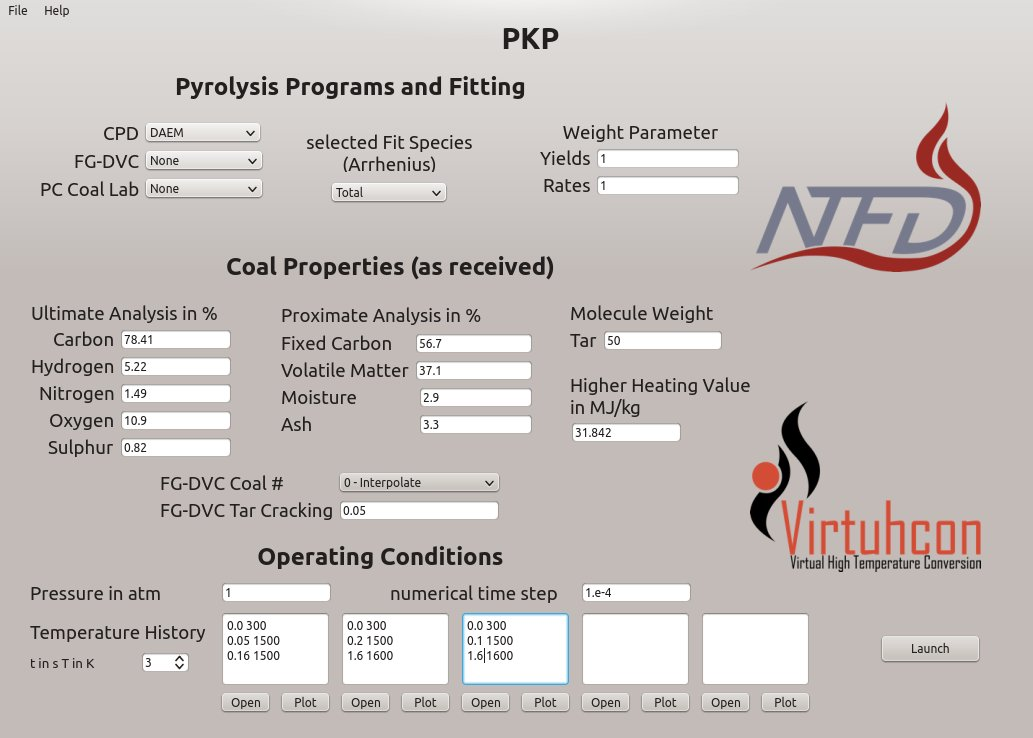
\includegraphics[width=14cm,angle=0]{Figures/GUI}
\caption{A screenshot of the Input GUI.}
\label{F_GUI}
\end{figure}

When starting the graphical user interface, file \emph{PKPgui.py}, the central input windows opens, see figure~\ref{F_GUI}.
As also visible in this figure, the general input structure is splitted into three parts: \emph{Pyrolysis Programs and Fitting}, \emph{Coal Properties} and~\emph{Operating Conditions}. The following selections can be done in the first of these:
\begin{itemize}
 \item \textbf{CPD}, \textbf{FG-DVC}, \textbf{PC Coal Lab}: These column boxes allow a selection, which of these detailed models shall be used and which kinetic parameter shall be fitted. The first two possible selections are here \emph{None}, for not running this model, \emph{Run} to just run it and make the species analysis. A fitting of kinetic parameter will not be carried out. Additional selections for fitting the results are \emph{constant~Rate}~(eq.~\ref{E_Reaction_g}), \emph{Arrhenius}~(eq.~\ref{E_Arrhenius_g}), \emph{Arrhenius~no~B}~(eq.~\ref{E_Arrhenius_g_noB}), \emph{Kobayashi}~(eq.~\ref{E_Kobayashi}) and \emph{DAEM}~(eq.~\ref{E_DAEM}). Here the fitting and the species analysis will be done.
 \item \textbf{selected Fit Species (Arrhenius)} is only important if one of the selected models to fit is \emph{Arrhenius} or \emph{Arrhenius~no~B}. This column box allows which species shall be fitted. Possible options to choose are here:
 \begin{itemize}
  \item \emph{Total}: only the overall yield is fitted
  \item \emph{Main Species}: the yield curves of the overall yields, tar and gas~(the sum of the light gases) are fitted
  \item \emph{all Species}: the kinetic parameter for all species outputted by the detailed model are fitted
 \end{itemize}
 \item \textbf{Weight Parameter} Enter the parameter for the fitting procedure. The text line Weight Parameter Yields sets the factor $\mathrm{a_0}$ in equation~\ref{E_Weight_Param1}, Rates sets $\mathrm{a_1}$ in equation~\ref{E_Weight_Param2}.
\end{itemize}
The second section of the GUI, the information about the coal can be entered. All properties refer to the coal in the as received state.
\begin{itemize}
 \item \textbf{Ultimate Analysis in ~\%} Sets the ultimate analysis of the coal. Values should be in percent.
 \item \textbf{Proximate Analysis in~\%} Sets the proximate analysis of the coal. Values should be in percent.
 \item \textbf{Molecule Weight Tar}: define the molecule weight of the tar. Required for the species analysis.
 \item \textbf{Higher Veating Value} Enter here the higher heating value of the coal in $\mathrm{\frac{MJ}{kg}}$.
 \item \textbf{FG-DVC Coal \#} FG-DVC needs an information whether the coal property file should be interpolated using the van-Krevelen~Diagram (option \emph{0-Interpolate}) or if a library coal should be used (1-8). If the selected coal is out of the range of the library coals, the closest library coal has to be selected. The generation of the coal file is also done automatically by PKP.\footnote{Using the FG-DVC \emph{coalsd.exe}. For more information see the FG-DVC manual.}
 \item \textbf{FG-DVC tar cracking} Defines the FG-DVC modeling of the tar cracking. Possible selections are:
 \begin{itemize}
  \item \emph{0.0} No tar cracking is modeled.\footnote{The option recommended by the FG-DVC manual~\cite{FGDVC_822}.}
  \item When entering a time in seconds, e.g. '0.01', defines the holding time of the tar in the coal molecule. The tar is cracked during this time frame.
  \item A negative number, e.g. '-1', sets the full tar cracking.
 \end{itemize}
\end{itemize}

The last section in the GUI allows the input of the operating conditions:
\begin{itemize}
 \item \textbf{Pressure in atm} Defines the pressure where the devolatilization occurs.
 \item \textbf{numerical time step} Sets the time step. For FG-DVC the constant value, for CPD the maximum.
 \item \textbf{Temperature History} With the spin box on the left, the numbers of temperature histories to apply is defined. If this is set to '3', three runs are carried out using the first three temperature histories. These temperature histories can be imported via the five text fields on the right. There the temperature histories can be entered manually or also be imported using the 'open' buttons in below. Additionally they can be plotted (button 'plot'). Using this option also saves the temperature history in a file~\emph{TempHist1.dat}.Where the number stands for the current field. These saved temperature histories can be re-imported using the 'open' button.\\
 All the temperature histories have to be entered in two columns, just separated by spaces. The time is in seconds, the temperature in Kelvin.
\end{itemize}

The head menu contains under File following options:
\begin{center}
\begin{tabular}{ll}
Write into Table & Ctrl+S\\
Write and Run & Ctrl+R\\
Load saved state & Ctrl+O\\
Show generated Results & Ctrl+T\\
Exit & Ctrl+Q\\
\end{tabular}
\end{center}
Where the Write saved all information into the \emph{.inp} files and the \emph{TempHist\#.dat} in the main directory. 'Load saved state' transfer this information into the current GUI.\\
The 'Write and Run' is identical with the button 'Launch' in the lower right of the GUI.\\
The file menu 'Help' offers to open this manual.\\

Please do not forget to make the general settings in the input files, before using PKP the first time, see chapter~\ref{SS_1stSteps}.\\

After running the result windows opens, figure~\ref{F_GUIDone}. It lists all calculated species in the column bar. With 'Show results' the yields over time for the detailed model output and the fitted equation are plotted. 'Open Species analysis' opens the textiles with the species analysis results for each run. Open kinetic parameter opens the text file with the results of the fitting, one file for each detailed model. If this window was closed, it can be reopened by the option 'Show generated Results'~(Ctrl+T) in the Main window. \\
All results are located in the Result directory. When starting a new run, its content is deleted.\\

\begin{figure}
\centering
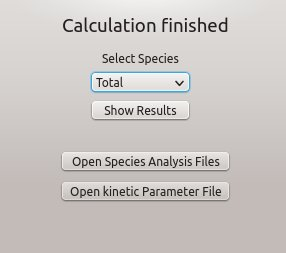
\includegraphics[width=4cm,angle=0]{Figures/GUI_Done}
\caption{A screenshot of the Result GUI.}
\label{F_GUIDone}
\end{figure}

\subsubsection{Using the input files}\label{SSS_inp}
The manual user input is managed by the four \emph{*.inp} files, \emph{Coal.inp, CPD.inp} \emph{FGDVC.inp} and \emph{OperCond.inp}.\\
The information you want to insert into these files have to be in the line below the line asking for the information. For example:\\

\noindent \emph{Fixed Carbon:\\
43.7}\\

This sets the amount of Fixed Carbon equal 43.7. The position~(i.e. the line) of such two lines in the input file does not matter, the only important point is the specific string~(in this example~\emph{Fixed Carbon:}) and that the value you want to set is in the following line after the string.\footnote{If you want to use another string in this file, you also have to change the individual file note in \emph{InformationFiles.py}.}\\
Firstly you will get a short overview into these files and the values to enter into them:\\
\paragraph{Coal.inp} contains the main information about the coal. PKP forwards the information about the coal from this file to the programs \CPD and the \FGDVC coal generator (\textit{/COALS/coalsd.exe} in the \FGDVC directory). The proximate analysis values are only required by \texttt{CPD}.
\begin{itemize}
 \item \textbf{Fixed Carbon:} sets the amount of fixed carbon in the coal. The value has to be entered in percent for a non-daf coal.
 \item \textbf{Volatile Matter:} sets the amount of volatile matter in the coal in percent, as received.
 \item \textbf{UA Carbon:}, \textbf{UA Hydrogen:}, \textbf{UA Nitrogen:}, \textbf{UA Oxygen:} sets the ultimate analysis for the coal to model. The values have to be entered in percent.
 \item \textbf{Higher Heating Value, as received, in J/kg:} sets the higher heating value for the coal. If this value is not known, set it equal zero. Then the Dulong formula~(equation~\ref{E_Dulong}) will be used to calculate the higher heating value.
 \item \textbf{Tar Molecule weight, MTar:} Sets the molecule weight of the tar, as it is required for the species and energy calculation, see chapters~\ref{SSS_ConsEqCPD}~and~\ref{SSS_ConsEqFGDVC}.
 \item \textbf{Weight-Parameter yields for fitting the kinetics:} sets the weight $\mathrm{a_0}$ of the equation~\ref{E_Weight_Param1} to weight the yields in the fitting procedure~(equation~\ref{E_LS}).
 \item \textbf{Weight-Parameter rates for fitting the kinetics:}  sets the weight $\mathrm{a_1}$ of the equation~\ref{E_Weight_Param2} to weight the rates in the fitting procedure~(equation~\ref{E_LS}).
\end{itemize}

\paragraph{CPD.inp} controls the \CPD program and the further work with its output.
\begin{itemize}
 \item \textbf{useCPD?:} if set to \emph{yes} or \emph{true}, \CPD will be launched.
 \item \textbf{selected fitting Approximation:} if the \emph{constantRate} is selected, the fitting will be carried out using equation~\ref{E_constRate_s}~and~\ref{E_constRate_g}. When selecting \emph{Arrhenius}, the kinetic parameter for the Arrhenius equation modeled pyrolysis kinetics~(equation~\ref{E_Arrhenius_g}) will be calculated. To fit the Kobayashi parameter, set it to \emph{Kobayashi}. If selecting \emph{None}, no fitting of the kinetic parameter will be carried out, just the direct \CPD results and species and energy balance will be generated.
 \item \textbf{initial time step in s:} The initial time step, \CPD starts to calculate with.
\item \textbf{print increment, writeValue:} Integer which sets the frequency of writing the result into the \texttt{CPD}-output file. E.g. '1' means every value is written into the file, '3' only every third value.
\end{itemize}

\paragraph{FGDVC.inp} controls the \FGDVC program and the further work with its output.
\begin{itemize}
 \item \textbf{use FG-DVC?:}  if set to \emph{yes} or \emph{true}, \FGDVC will be launched.
 \item \textbf{selected fitting Approximation:} This selection is analogous to the in \textit{CPD.inp}
 \item \textbf{main directory FG-DVC:} sets the main path of \texttt{FG-DVC}, where the \emph{fgdvc.exe} is located. One example: '{C:\verb|\|Programs\verb|\|FGDVC\_8-2-3\verb|\|}'
 \item \textbf{directory fgdvc-output:} Sets the main directory, where \FGDVC outputs the results. This is in general the directory, where the \emph{fgdvcd.exe} is located. One example: '{C:\verb|\|Programs\verb|\|FGDVC\_8-2-3\verb|\|FGDVC\verb|\|}'.\\To use other already generated FG-DVC output files, it is a good option to set their path here. As long as they are still named \emph{gasrate.txt} and \emph{gasyield.txt}, the fitting will be carried out on the information contained in these files.
 \item \textbf{Choose Coal:} If this is set equal \emph{0}, the interpolation of the coal will be carried out using the information from \emph{Coal.inp} and the FG-DVC program \emph{coalsd.exe}, leading to specific \FGDVC coal files for the applied coal. If the file cannot be generated, i.e. the used coal is outside the interpolation triangle\footnote{see the FG-DVC manual for more details: THE FG-DVC COAL PYROLYSIS MODEL USER'S GUIDE Version 8.2.3 for Windows; Advanced Fuel Research, Inc., 87 Church Street, East Hartford, CT 06108-3728, USA; 2012}, select a value from \emph{1}~to~\emph{8} to use one of the \FGDVC library coals. The order here is the same as in \texttt{FG-DVC}:
 \begin{enumerate}
  \item Beulah-Zap
  \item Wyodak-Anderson
  \item Illinois \# 6
  \item Bind Canyon, UT
  \item Lewis-Stockton, WV
  \item Pittsburgh \# 8
  \item Upper Freeport, PA
  \item Pocahontas \# 3, VA
 \end{enumerate}
 \item \textbf{Model tar cracking?} To model no tar cracking~(as recommended in the \FGDVC manual) set the tar residence time equal \emph{0}. A partial tar cracking can be modeled by set the tar residence time is seconds. If a full tar cracking shall be used, set the residence time to a negative input value, e.g write \emph{-1}.           
\end{itemize}

\paragraph{OperCond.inp} sets the operating condition for the pyrolysis programs.
\begin{itemize}
  \item \textbf{pressure in atm:} Sets the constant pressure in atmospheres.
 \item \textbf{FG-DVC: constant (numerical) time step; CPD: maximum time step}: Enter here the numerical time step, the constant for \FGDVC and the maximum value for \texttt{CPD}.
 \item \textbf{Number of Temperature Histories to include:} Defines, how many runs of the pyrolysis  models should be carried out. The different temperature history will be defined with the help of the next point:
 \item \textbf{Start Time History 1:} This line have to follow two columns, defining the temperature history for the first run of the pyrolysis models. The first column lists the time in seconds, the second one the temperature in K. The last time point is automatically selected as the final pyrolysis time. The end of the time-temperature array has to be labeled by the term \emph{End Time History 1}. Here one example:\\
\emph{Start Time History 1\\
0, 293\\
0.05, 1000\\
0.1, 1700\\
0.6, 1700\\
End Time History 1\\}
Analogue to this term the numbers 2~to~5 label the temperature history for the second to the fifth run.
\end{itemize}


\subsubsection{The Result Files}\label{SSS_ResultsFiles}
The generated results are documented in the following files. The name of the text-files contains in front the used pyrolysis program (e.g. \emph{CPD-BalanceResults.txt}).

\paragraph{BalanceResults.txt}
This file contains the output of the species and the energy conservation, chapters~\ref{SSS_ConsEqCPD}
~and~\ref{SSS_ConsEqFGDVC}. The first part lists the input of the UA, PA and HHV. Afterwards, the final yields of all species are enumerated, as the result of using the equation~\ref{E_add_up}~to~\ref{E_MethanNew}. The tar composition~(equation~\ref{E_TarComp}), assuming a $\mathrm{C_nH_mO_p}$ molecule with an average molecule mass, inputted by the user, is given by the factors n, m, p. The last two parts show the results applying the equations~\ref{E_Dulong}~to~\ref{E_QPyro}.

\paragraph{Results\_const\_rate.txt}
This file contains the kinetic parameters for the constant rate (equation~\ref{E_constRate_s}~or~\ref{E_constRate_g}) fitting. The two parameters are k in $\mathrm{\frac{1}{s}}$ and $\mathrm{t_{start}}$ in s.

\paragraph{Result\_ArrheniusRate.txt}
\emph{Result\_ArrheniusRate.txt} lists all kinetic parameter~(A in $\mathrm{\frac{1}{s}}$ and E~in~K) for the Arrhenius equation~\ref{E_Arrhenius_s}~or~\ref{E_Arrhenius_g}.

\paragraph{Results\_KobayashiRate.txt}
This file list for all species the Kobayashi kinetic parameter $\mathrm{A_1 \; and \; A_2 \; in \; \frac{1}{s}}$, $\mathrm{E_1 \; and \; E_2 \; in \; K}$, $\mathrm{\alpha_1 \; and \; \alpha_2}$.

\paragraph{Fit\_result\_[Species]\_[R/Y].pdf}
These files contains the plots of the pyrolysis program output curve and the estimated curve using the applied model. These plots show the rate (then *\_R.pdf) or yields (*\_Y.pdf). This plot exists for all species calculated by the pyrolysis program (named in *\_Species\_*).

\paragraph{Fit\_result\_[Species].out}
For every species is in the referring file the \emph{Time}, \emph{Temperature}, \emph{Yields} and the \emph{Rates} written in columns. This is not the original output from the pyrolysis program, it is the result applying the selected equation with the fitted parameter.


\section{Equations}\label{S_Eq}

\subsection{Pyrolysis Kinetic Equations}\label{SS_KinEq}
In PKP are four possible kinetic models to select:
\begin{itemize}
 \item The Constant Rate Model, section~\ref{SSS_cR}
 \item The Arrhenius Model, \ref{SSS_Arrh}
 \item The Kobayashi Model, \ref{SSS_Kob}
 \item The Distributed Activation Energy Model, \ref{SSS_DAEM}
\end{itemize}
The Kobayashi model has the advantage, that the yields are dependent on the individual temperature history. A change, may in in the final temperature leads to a higher yield.\\
The constant rate and the Arrhenius model has fixed final yields. The general devolatilization reactions for these two models are described with equations~\ref{E_Reaction_s}~and~\ref{E_Reaction_g}, where~\ref{E_Reaction_s} describes the mass loss of the solid~(index~\textit{s}) coal, equation~\ref{E_Reaction_g} the formation of the yields~(gaseous:\textit{g}, individual:\textit{i}).
\begin{align}
\label{E_Reaction_s}
 \frac{dm_{s}}{dt}&=-k_s \: \left( m_{s} - m_{s,final} \right)\\
\label{E_Reaction_g}
 \frac{dm_{g,i}}{dt}&=k_{g,i} \: \left(m_{g,i,final} - m_{g,i}\right)  
\end{align}
So when using more than one run, also the final yield is a parameter to fit. It will be located in between the final yields of the runs of the pyrolysis models.

In the following subsections, the plots showing the rates and yields were generated with \CPD and \FGDVC showing the yields and rates for different species. All are based on the same temperature profiles as shown in figure~\ref{F_Tt}.
\begin{figure}
\centering%\capstart
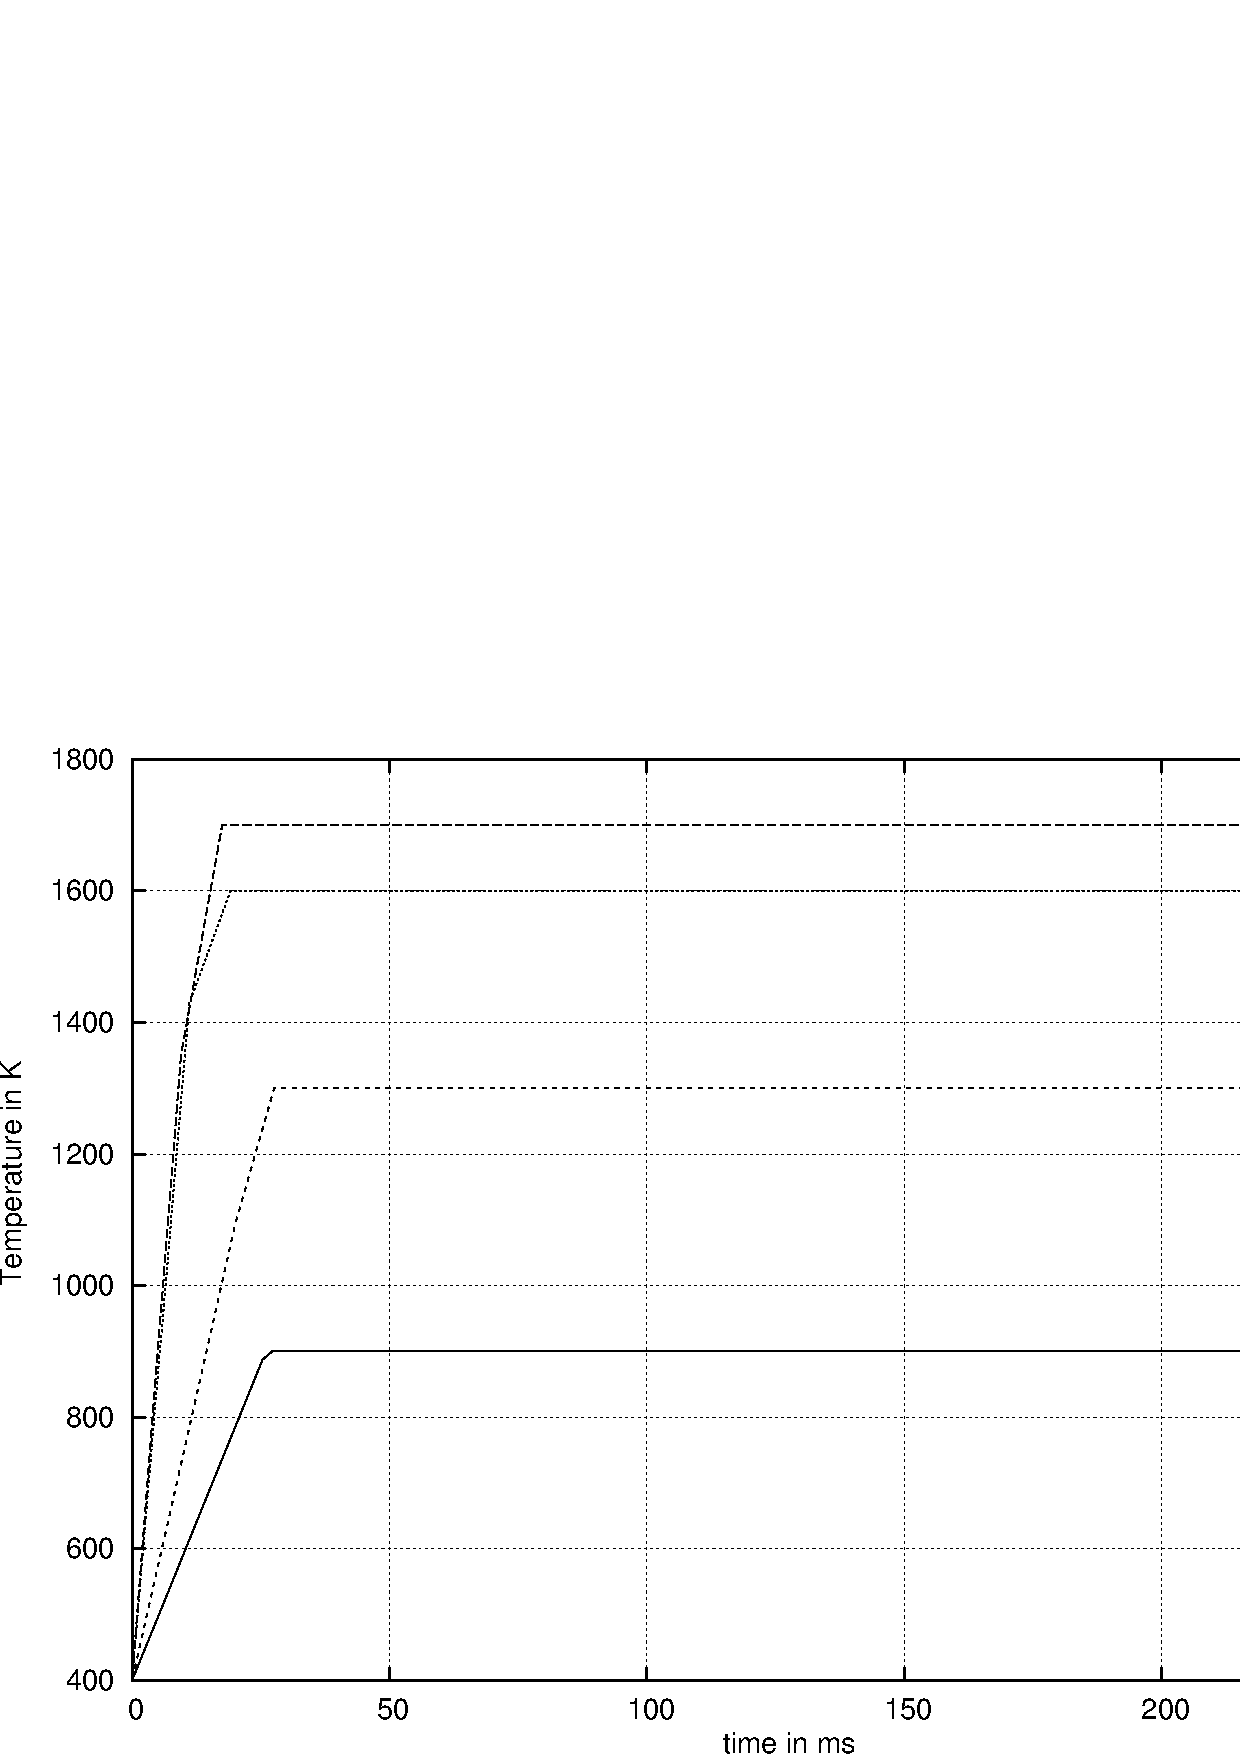
\includegraphics[height=8cm,angle=0]{Figures/tempHist}
\caption{The temperature history.}
\label{F_Tt}
\end{figure}

The table~\ref{T_Fit} gives an overview of the models with their parameters to fit and species to apply this model on. This is described more detailed in the next subsections.

\begin{table}
\newcommand{\mc}[3]{\multicolumn{#1}{#2}{#3}}
\begin{center}
\label{T_Fit}
\caption{The fitted models and their parameter.}
\begin{tabular}{lll}\hline
\textbf{Model} & \textbf{fitted parmeter} & \textbf{fitted species}\\\hline
constant Rate & \mc{1}{c}{$k_i$, $t_{start,i}$, $m_{final}$} & \mc{1}{c}{all}\\
Arrhenius & \mc{1}{c}{$A_i$, $b_i$, $E_i$, $m_{final}$} & \mc{1}{c}{all}\\
Kobyashi & \mc{1}{c}{$A_1$, $E_1$, $A_2$, $E_2$} & \mc{1}{c}{total}\\
DAEM & \mc{1}{c}{ } & \mc{1}{c}{ }\\\hline
\end{tabular}
\end{center}
\end{table}


\subsubsection{The Constant Rate Model}\label{SSS_cR}

Assuming a \textbf{constant rate} ($\mathrm{k = const. }$ and a starting time $\mathrm{t_{start}}$), the equations~\ref{E_Reaction_s}~and~\ref{E_Reaction_g} can be solved analytically:
\begin{align}
\label{E_constRate_s}
m_s(t)&=m_{s,final} + \left( m_{s}(t=t_{start,s}) - m_{s,final} \right) \: e^{-k_s(t-t_{start,s})}\\
\label{E_constRate_g}
m_{g,i}(t)&=m_{g,i,final}\cdot \left( 1 - \: e^{-k_i(t-t_{start,i})} \right)\\
\label{E_Offset_Time}
if \;\;\; t\leq t_i\::\;\;\; m(t)&=m(0)
\end{align}

This leads to advantage concerning the computational costs. On the other hand is this model completely independent from the temperature history. This is visualized in figure~\ref{F_Fit_cR_Y} where all fitted curves overlap each other.\\
The parameters to fit are for every species:
\begin{itemize}
 \item the starting time~($t_{start,i}$), where the devolatilization begins
 \item the constant rate factor $k_i$
 \item the final yield (when more than one run)
\end{itemize}
This model is applied to all species.

\begin{figure}
\centering%\capstart
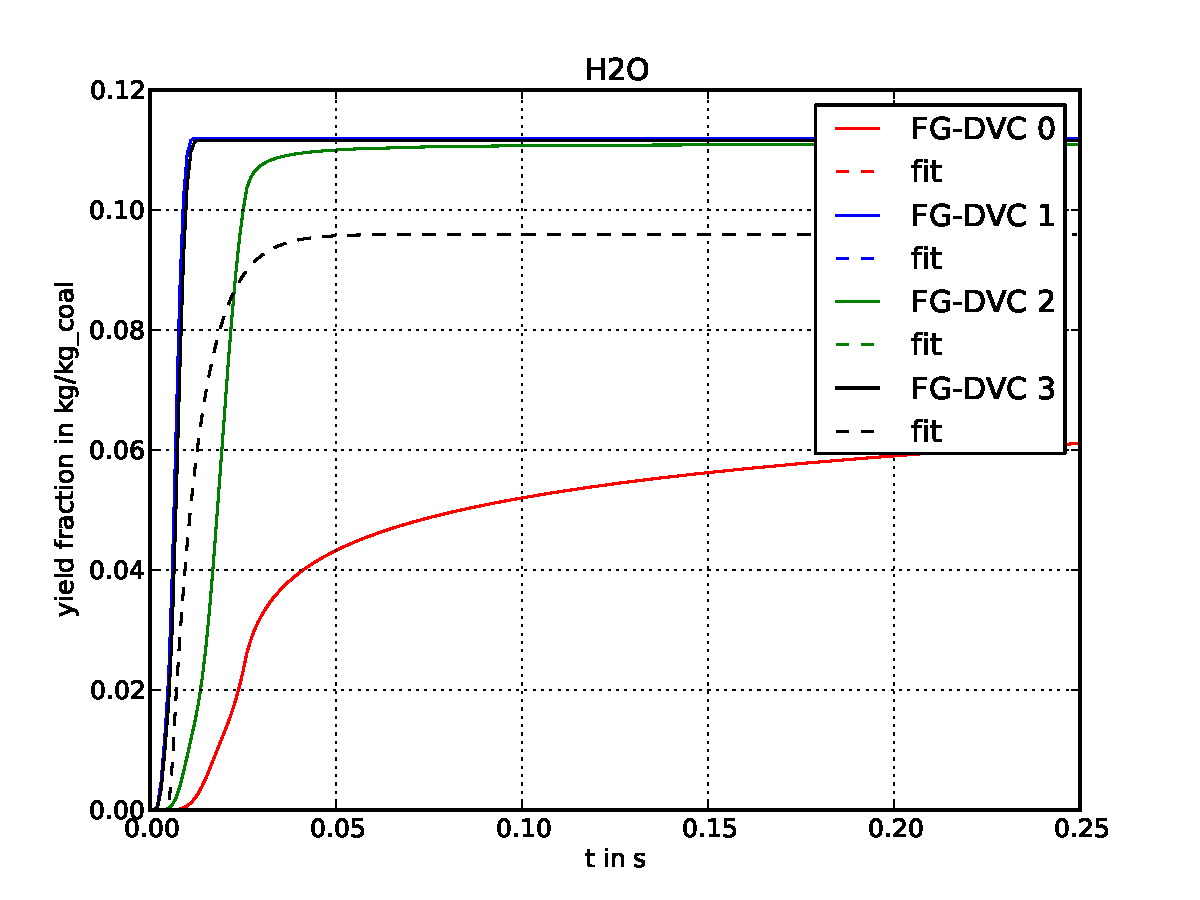
\includegraphics[height=9cm,angle=0]{Figures/FG-DVC-Fit_result_cR_H2O_Y}
\caption{One fitting result (Yields) for the constant Rate Model. The observed species is water.}
\label{F_Fit_cR_Y}
\end{figure}

%\begin{figure}
%\centering%\capstart
%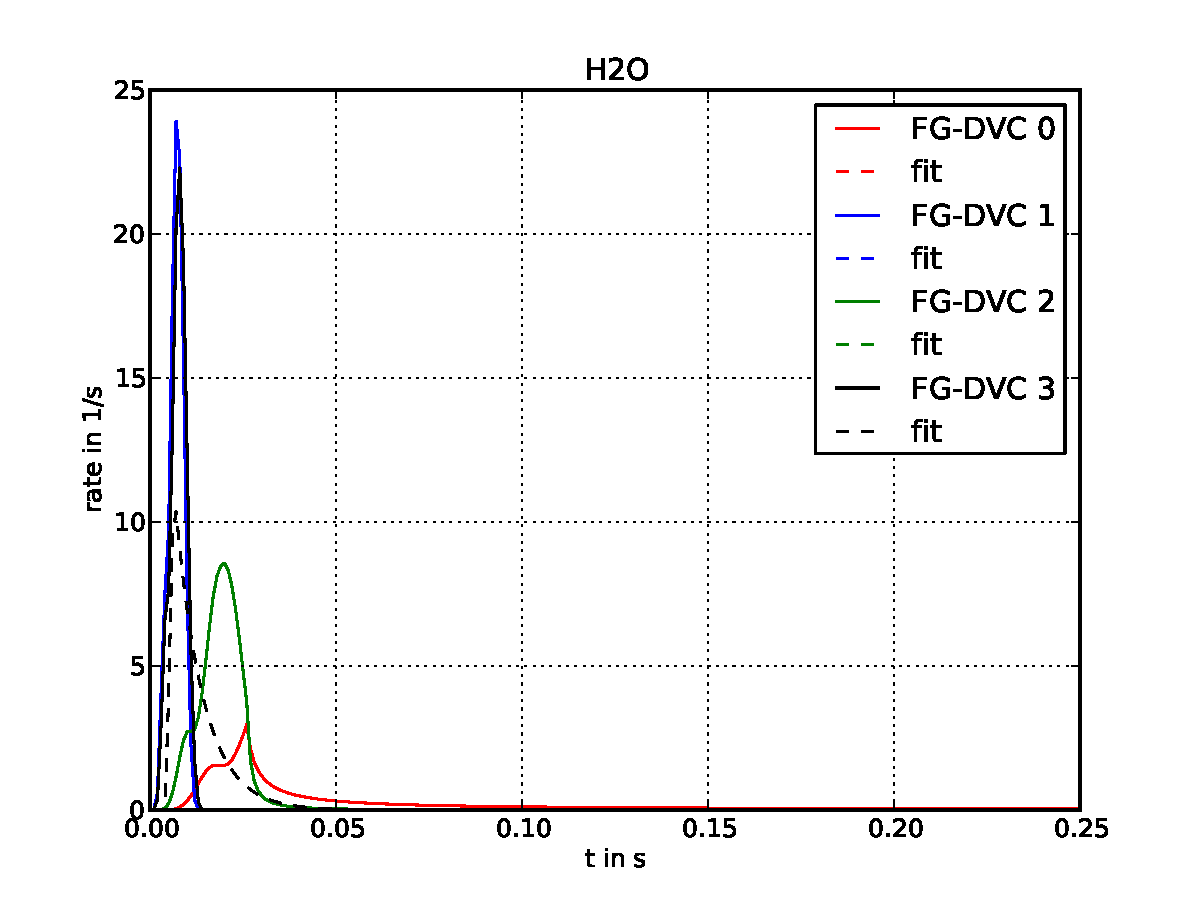
\includegraphics[height=9cm,angle=0]{Figures/FG-DVC-Fit_result_cR_H2O_R}
%\caption{One fitting result (Rates) for the constant Rate Model. The observed species is water.}
%\label{F_Fit_cR_R}
%\end{figure}

\subsubsection{The Arrhenius Model}\label{SSS_Arrh}

The kinetic rate k can be also expressed with the \textbf{Arrhenius} equation:
\begin{align}\label{E_Arrhenius_s}
 \frac{dm_s}{dt}&=A_s \cdot T(t)^{b_s} \cdot e^{-\frac{E_s}{T(t)}}\left( m_{s} - m_{s,final} \right)\\
\label{E_Arrhenius_g}
 \frac{dm_{g,i}}{dt}&=A_i \cdot T(t)^{b_{g,i}} \cdot e^{-\frac{E_{g,i}}{T(t)}}\left(m_{g,i,final} - m_{g,i}\right)
\end{align}
This notation of the Arrhenius equation includes no gas constant R in the exponential term. So the activation energy (or here more precise activation temperature) has the unit Kelvin. This is so far an advantage as the fitted $E_i$ is independent of the used unit system~(SI or cgs).\\
A second notation of the Arrhenius equation contains not the correction term $T(t)^{b_{g,i}}$:
\begin{align}\label{E_Arrhenius_s_noB}
 \frac{dm_s}{dt}&=A_s \cdot e^{-\frac{E_s}{T(t)}}\left( m_{s} - m_{s,final} \right)\\
\label{E_Arrhenius_g_noB}
 \frac{dm_{g,i}}{dt}&=A_i \cdot e^{-\frac{E_{g,i}}{T(t)}}\left(m_{g,i,final} - m_{g,i}\right)
\end{align}

Unlike the constant rate model is the Arrhenius modeled rate influenced by the temperature. But the Arrhenius model can be used to express the evolve for all species and the final yields are also fixed. So the parameter to fit are here:
\begin{itemize}
 \item the preexponentiation factor~$A_i$
 \item the correction factor $b_i$
 \item the activation energy $E_i$
 \item the final yield (when more than one run)
\end{itemize}
This model is applied to all species.\\

The Arrhenius model leads to a good agreement in the yield and rate curves for a limited range of temperatures, figures~\ref{F_Fit_Arrh_Y},~\ref{F_Fit_Arrh_R}. The disadvantage is the temperature independent yield fraction, all integrals for the rate curves in figure~\ref{F_Fit_Arrh_R} are the same. This leads to an imprecision as the yields show a dependency on the final temperature and heating rate.


\begin{figure}
\centering%\capstart
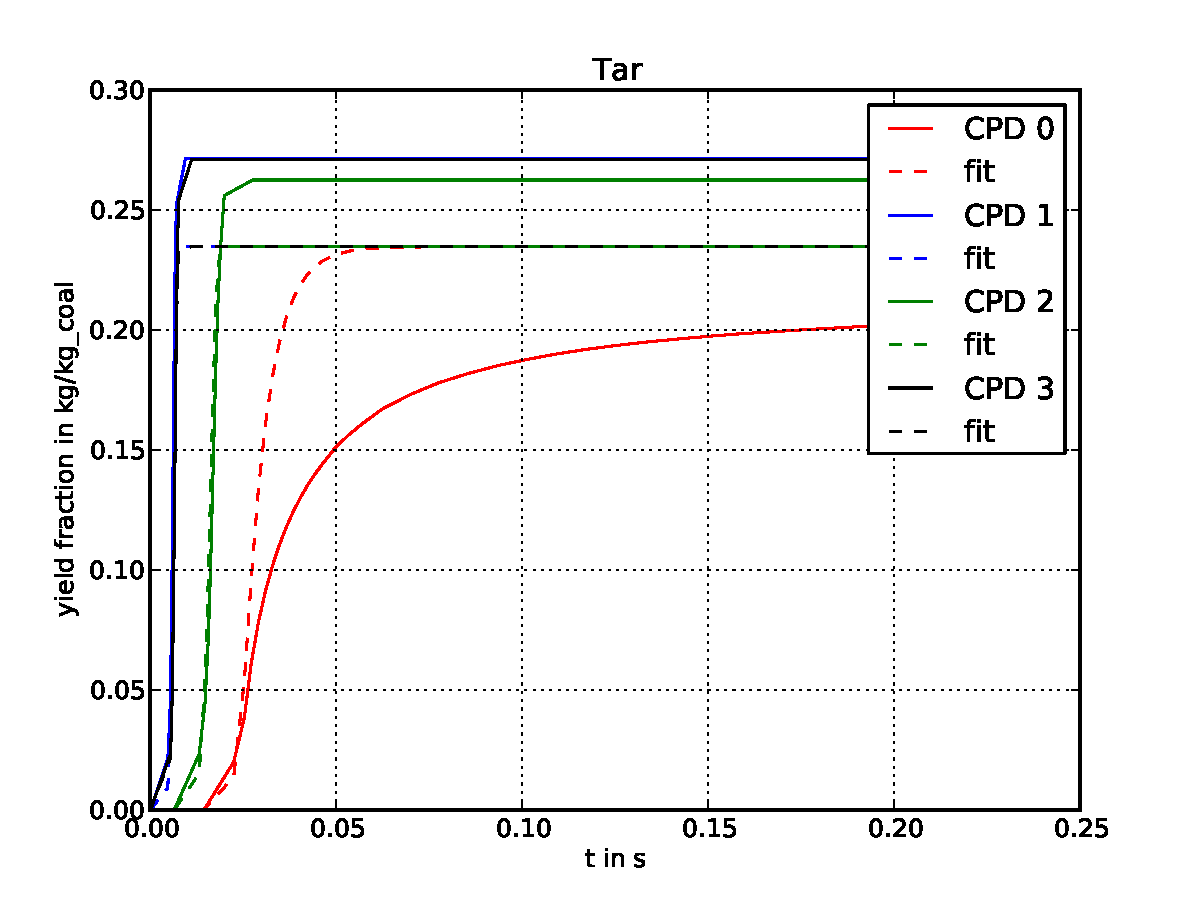
\includegraphics[height=9cm,angle=0]{Figures/CPD-Fit_result_Arrh_Tar_Y}
\caption{One fitting result (Yields) for the Arrhenius Model. The observed species is tar.}
\label{F_Fit_Arrh_Y}
\end{figure}

\begin{figure}
\centering%\capstart
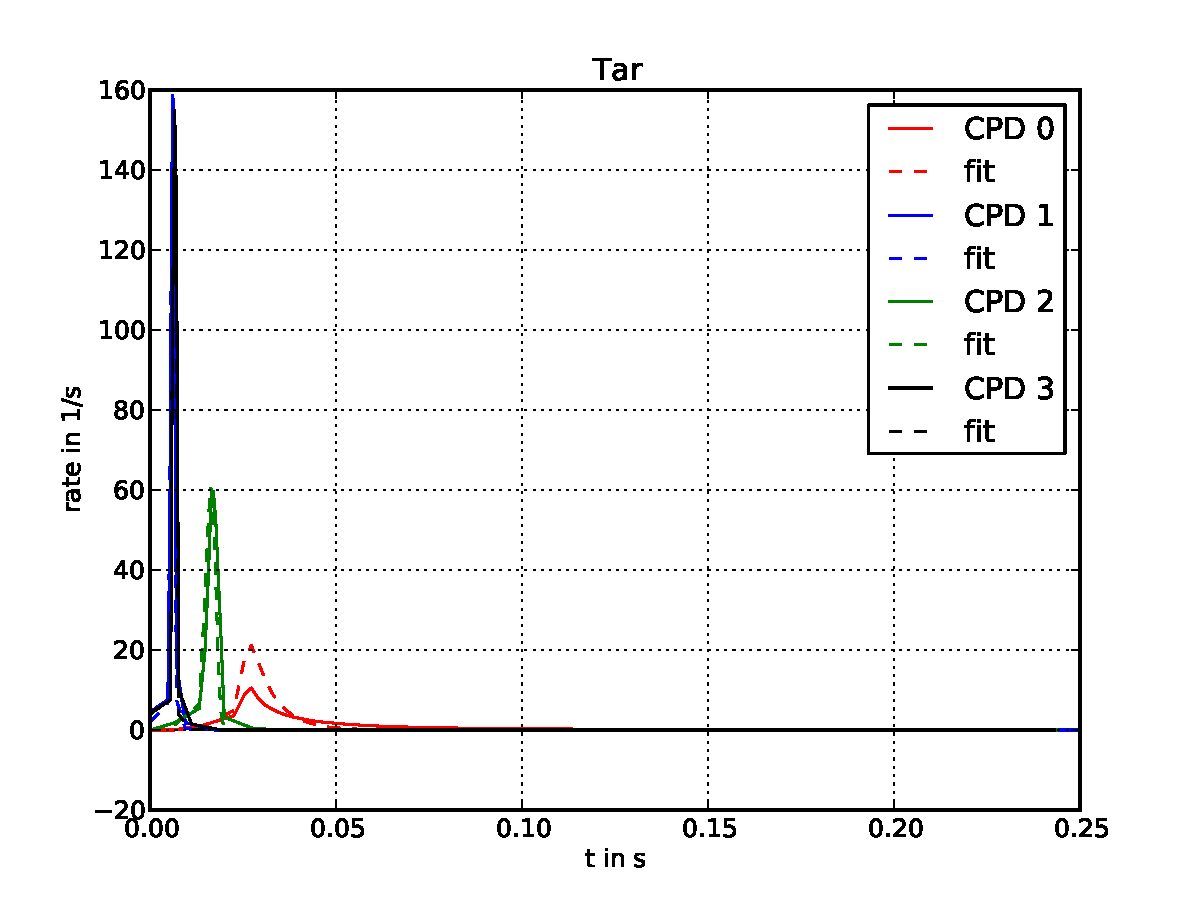
\includegraphics[height=9cm,angle=0]{Figures/CPD-Fit_result_Arrh_Tar_R}
\caption{One fitting result (Rates) for the Arrhenius Model. The observed species is tar.}
\label{F_Fit_Arrh_R}
\end{figure}

\subsubsection{The Kobayashi Model}\label{SSS_Kob}

Also the \textbf{Kobayashi} equation, also Two Competing Reaction Model, can be fitted, see equation~\ref{E_Kobayashi}. The optimization is carried out using the Arrhenius notation of equation~\ref{E_Kob_k} for $\mathrm{k_1}$ and $\mathrm{k_2}$.
\begin{equation}\label{E_Kobayashi}
 \frac{m_v(t)}{m_{p,0} - m_a}= \int_{0}^{t} ( \alpha_1 k_1 + \alpha_2 k_2 ) exp \left( -  \int_{0}^{t} ( k_1 + k_2 ) \; dt \right) \; dt
\end{equation}
\begin{equation}\label{E_Kob_k}
 k_j=A_j \:e^{-\frac{E_{j}}{T(t)}} \;\;\;\;\;\; with \: j=1,2
\end{equation}

The Kobayashi model can be applied only on the the overall, the total yields. The yield of individual species could be generated by multiplying the overall yield with the yield fraction~$\frac{y_i}{y_{all}}$. But as the composition of the yields varies with the temperature history this factor also shows this dependency, which may leads to an imprecision when modeling the individual yields.\\
The final yields of this model are dependent on the temperature, see figures~\ref{F_Fit_Kob_Y}~and~\ref{F_Fit_Kob_R}. The range of the yields are defined by the two weight factors~$\alpha_1$~and~$\alpha_2$. The $k_1$ models the reactions at lower temperatures~(low $A_1$ and $E_1$), $k_2$ at higher temperatures~(high $A_2$ and $E_2$). If the final temperature has very low values, the yields will converge to~$\alpha_1$. If the temperatures will raise to infinity, the yields will be equal~$\alpha_2$. So $\alpha_2$ is ever set equal one: $\alpha_2=1$. $\alpha_1$ is equal the amount of volatile matter in the daf coal. As the measurements, the proximate analysis of coal is based on, were carried out at very low heating rates compared with the ones occurring at gasification and combustion processes, the approximation $\alpha_1=VM$ is an applicable and good assumption.\\

For the fitting procedure, the inner integral $\int_{0}^{t} ( k_1 + k_2 ) \; dt$ is approximated by the Trapezoidal rule.\\

As it can be seen in figures~\ref{F_Fit_Kob_Y}~and~\ref{F_Fit_Kob_R}, the higher temperatures~(figure~\ref{F_Tt}) lead to higher yields. But the influence of the temperature cannot be modeled that the dependency on temperature is completely the same as in the output of the more complex pyrolysis programs. So leads the higher temperature in case~1 compared to case~3 to a slightly higher yield in the output of \CPD while the influence on the Kobayashi modeled result is greater.

\begin{figure}
\centering%\capstart
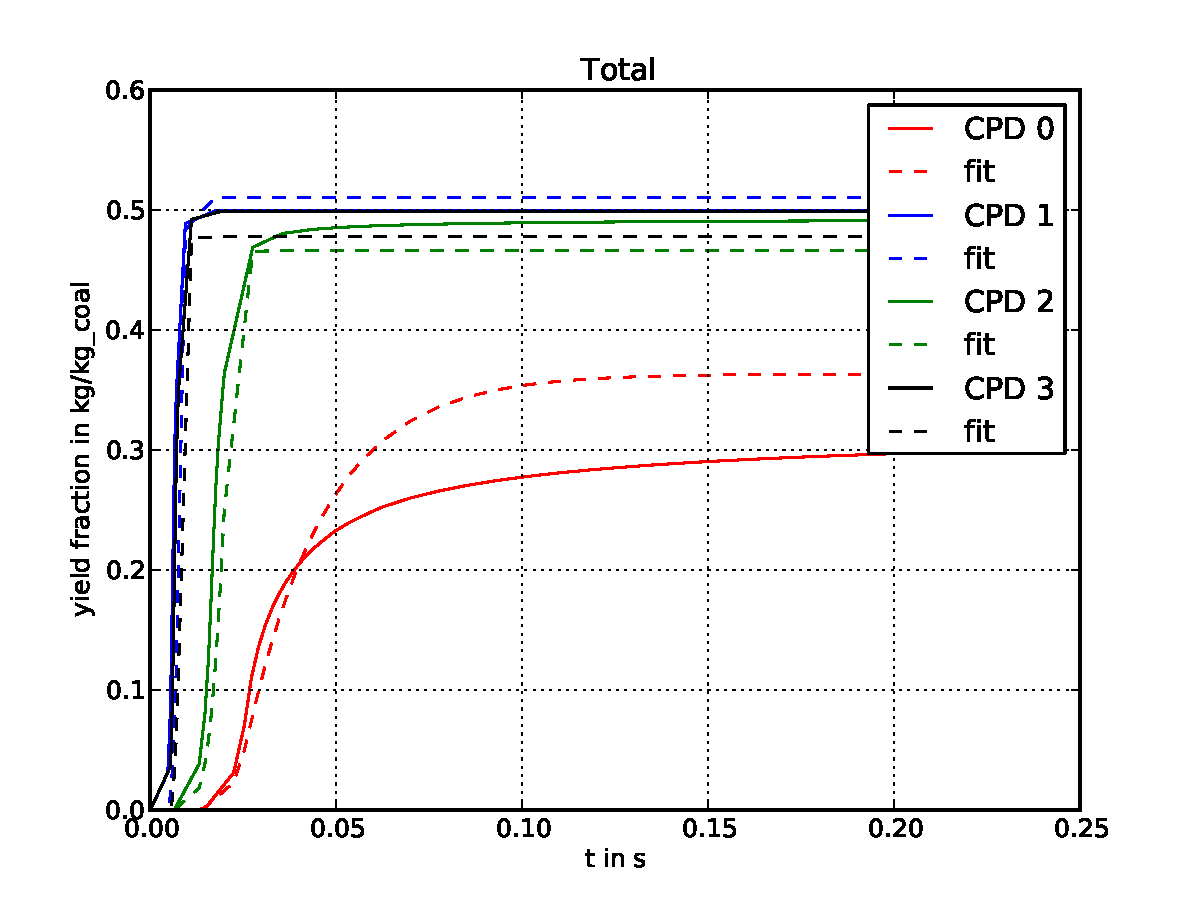
\includegraphics[height=9cm,angle=0]{Figures/CPD-Fit_result_Kob_Total_Y}
\caption{One fitting result (Yields) for the Kobayashi Model. The Kobayashi model just optimizes the overall yields.}
\label{F_Fit_Kob_Y}
\end{figure}

\begin{figure}
\centering%\capstart
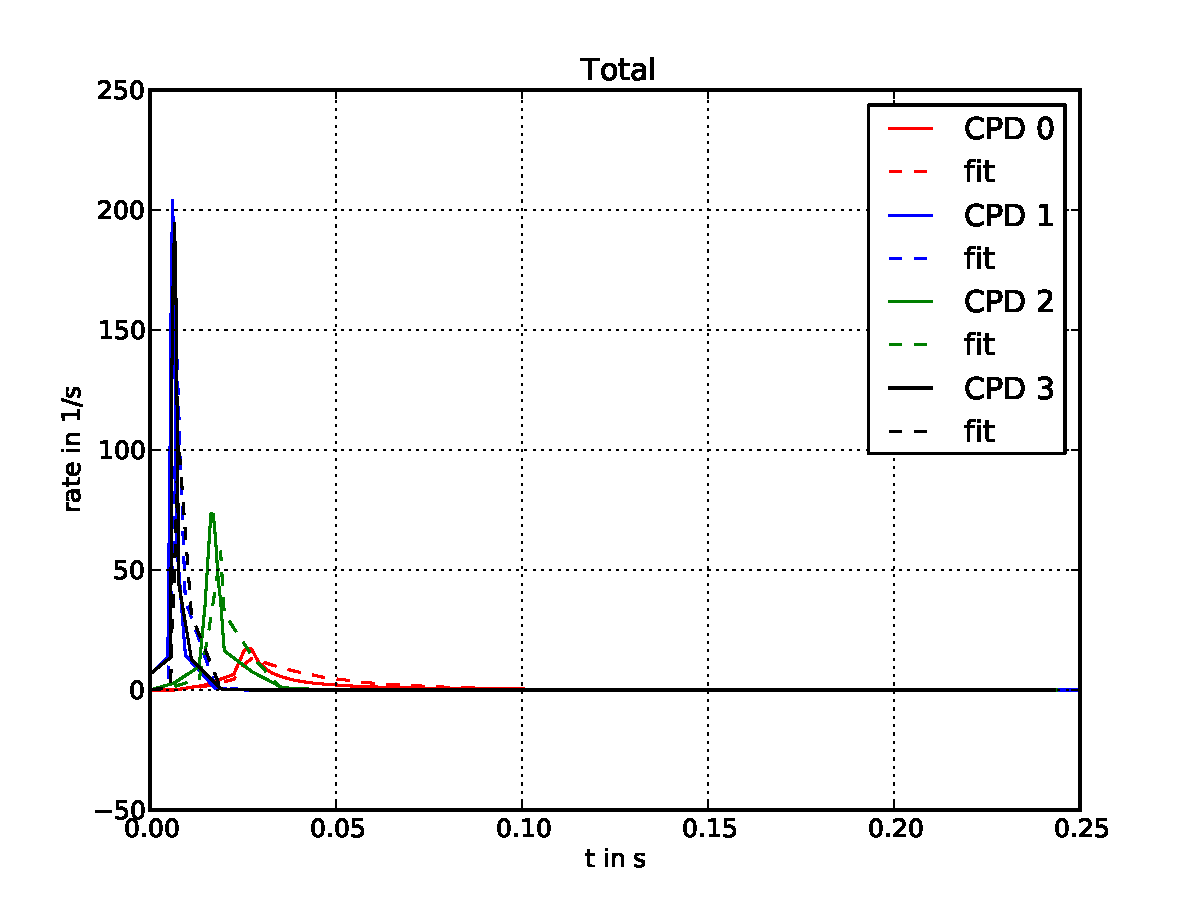
\includegraphics[height=9cm,angle=0]{Figures/CPD-Fit_result_Kob_Total_R}
\caption{One fitting result (Rates) for the Kobayashi Model.}
\label{F_Fit_Kob_R}
\end{figure}

\subsubsection{The Distributed Activation Energy Model}\label{SSS_DAEM}
The Distributed Activation Energy Model~(DAEM) considers parallel first order kinetics over a specific range, described by a distribution function~(F(E)). The equation used in PKP is:
\begin{equation}\label{E_DAEM}
 m = m_{final} \left( 1 - \int_{0}^{\infty} exp\left[ -A_0 \cdot \int^{t_{final}}_{t_0} exp\left( -\frac{E}{T} \right) dt  \right] F(E) \right)
\end{equation}
As a distribution function, a Gaussian Distribution is used:
\begin{equation}\label{E_GaussDistr}
 F(E) = \frac{1}{\sigma \cdot \sqrt{2\pi}} \cdot exp \left( -\frac{(E-E_0)^2}{2\sigma^2} \right)
\end{equation}
So there are four parameters to optimize:\\
\begin{enumerate}
 \item the preexponentiation factor $\mathrm{A_0}$, which is here equal for all reactions.
 \item $\mathrm{E_0}$, defining the center of the Gaussian Distribution
 \item and $\mathrm{\sigma}$, which spcifies the flattening of the Distribution curve and its range
 \item for multiple runs, the $\mathrm{m_{final}}$ also has to be optimized
\end{enumerate}
For solving the outer integral over dE, the Simpson tule is used. But for the nemuerical solution of the integral, the range has to be modified. As reported in the paper by Cai~\cite{Cai_DAEM1}, the integration boundaries can be se to $\mathrm{E_0 + 3 \cdot \sigma}$ as the upper and $\mathrm{E_0 - 3 \cdot \sigma}$ as the lower limit. This range covers up to 99.73~\% of the applied Gaussian Distribution. So for the further fitting of the devolatilization reaction, the prerequisite $\mathrm{E_0 > 3 \cdot \sigma}$ should be in force to achieve realistic results.\\
The inner integral $\mathrm{\int^{t_{final}}_{t_0} exp\left( -\frac{E}{T} \right) dt}$ was already simplyfied by setting $\mathrm{A_0}$ as a constant. In many papers~\cite{Cai_DAEM1,Cai_DAEM2,Cai_DAEM3,Slovak_DAEM} a linear heating rate over the whole time range is assumed, so $\mathrm{\frac{dT}{dt}=\beta}$. The transformation of the integral allows to integrate over the temperature. For such temperature integrals different analytical approaches exist~\cite{Cai_DAEM1,Cai_DAEM2}. This method was also tested.
 But as this is only a very specific case of the operating conditions and even not faster than solving the integrals\footnote{The reason might be that the very large analytical equations in Python (as an interpreting language) take more time than let the integral solve by a external library.}, this approach is furthernot considered. The double integral is solved numerically.\footnote{There are also other approaches to avoid the double integration like in the paper by McGuiness et al.~\cite{McGuiness_DAEM}, but also these assumptions made here ($\mathrm{\sigma \rightarrow 0 }$ or $\mathrm{\frac{E_0}{T} \rightarrow \infty }$) cannot be applied here.}\\
The outer integral is solved over a specific number of activation energies. For each activation energy the inner integral is solved and the value for all time steps saved, using a compisite Trapezoidal rule\footnote{the \texttt{scipy.integrate.cumtrapz} module, http://docs.scipy.org/doc/scipy/reference/generated/scipy.integrate.cumtrapz.html}. All inner integrals are saved in a 2D-Array($\mathrm{t_i,E_i}$). Each column contains all values of the inner integral for all time steps (the same activation energy), each line allinner integrals at the time $\mathrm{t_i}$. After this array is calculated, the equation of the outer integral is used for all values of the current line of the matrix and afterwards this list is integrated over dE.



\subsubsection{Fitting the Kinetic Equations}\label{SSS_FitKin}
The fitting procedure is carried out with a \texttt{scipy-optimizer}\footnote{\textit{http://docs.scipy.org/doc/scipy/reference/optimize.html}} \footnote{The standard setting optimizer is \texttt{fmin}.  The \texttt{leastsq} optimizer is the second choice.} and the \texttt{scipy.odeint}\footnote{\textit{http://docs.scipy.org/doc/scipy/reference/generated/scipy.integrate.odeint.html}} package to minimize the residual~$E(k,m_{fit})$ in the equation~\ref{E_LS}. For the structure of the whole fitting procedure see chapter~\ref{S_Program}. In equation~\ref{E_LS} is $\mathrm{m_{out}}$ the output of the devolatilization program \CPD or \FGDVC. The optimization is carried out over all points reported in the output file of the pyrolysis program. The normalized weight factor parameters~$\mathrm{a_0}$~and~$\mathrm{a_1}$ in the equations~\ref{E_Weight_Param1}~and~\ref{E_Weight_Param2} can both be defined by the user, the standard setting is for both one.

\begin{equation}\label{E_LS}
 E(k,m_{fit})=\omega_0 \int \left( m_{out}(t) - m_{fit}(k,t) \right)^2 dt \; + \; \omega_1 \int \left( \dot m_{out}(t) - \dot m_{fit}(k,t) \right)^2 dt
\end{equation}
\begin{align}
 \label{E_Weight_Param1}
\omega_0 &= \frac{a_0}{\left( max(m_{out})-min(m_{out}) \right)^2}\\
 \label{E_Weight_Param2}
\omega_1 &= \frac{a_1}{max(\dot{m}_{out}^2)}
\end{align}

\subsubsection{Pyrolysis Species- and Energy Conservation for \CPD output}\label{SSS_ConsEqCPD}

\paragraph{Species Conservation}
As the first step it has to be checked that the oxygen content in the generated yields~(oxygen containing species $\mathrm{f_i}$ with $\mu_i^{O}$ oxygen) is less equal that the oxygen in the ultimate analysis:
\begin{equation}
 UAO^{cpd, \: species \: output} = M_{O} \sum_i \frac{\mu_i^{O} f_i}{M_i} \le UAO 
 \label{E_O_balance}
\end{equation}
The factor~$\mathrm{\gamma}$~(\ref{E_gamma}) tells if the outputted yields contain less oxygen than reported in the Ultimate Analysis~(UA)~($\gamma > 1$) or if they are equal~($\gamma = 1$). For the case that~$\gamma < 1$, the oxygen containing yields have to be decreased by using equation~\ref{E_scale_up}, while the amount of the other species have to be increased to conserve the conserve the amount of volatile matter~(equation~\ref{E_add_up}). In this case, the tar will contain no oxygen. The yield of $N_2$ is equal to the UA of Nitrogen.

\begin{align}
 \gamma &= \frac{UAO}{UAO^{cpd, \: species \: output}}
 \label{E_gamma}\\
 f_i^{new} &= \gamma \cdot f_i 
 \label{E_scale_up}\\
 f_{oth}^{new} &= f_{oth} + \left(1-\gamma\right) \sum_i f_i
 \label{E_add_up}
\end{align}

For the case $f_{N_2}<f_{other}$, the remaining part is assigned to $CH_4$:

\begin{equation}
 f_{CH_4}^{new} = f_{CH_4} + \left( f_{oth}^{new} - f_{N_2} \right)
\label{E_MethanNew}
\end{equation}

Now the composition of tar can be calculated. For each element~C,H,O, the following equation~\ref{E_TarComp} can be used, assuming a tar composition of~$C_nH_mO_p$. $M_j$ is the atom weight of the element~j, $\mu_i^j$ the number of atoms of~$j$ in the species~$i$.

\begin{equation}
\frac{UA_j}{M_j} = \mu_{tar}^j \frac{f_{tar}}{M_{tar}} + \sum_i \mu_i^{j} \frac{f_{i}}{M_{i}}
%{UA_j} = \mu_{tar}^j \frac{f_{tar}}{M_{tar}} + \sum_i \mu_i^{j} \frac{f_{i}}{M_{i}}
\label{E_TarComp}
\end{equation}


\paragraph{Energy Conservation}
The Dulong formula is used, if the higher heating value~(HHV) of the coal is not known:
\begin{equation}\label{E_Dulong}
 HHV = 32.79 \cdot UAC + 150.4 \cdot (UAH - UAO/8) + 9.26 \cdot UAS + 4.97 \cdot UAO + 2.42 \cdot UAN
\end{equation}
where UAC, UAH, UAO, UAS and UAN are the value of the ultimate analysis for carbon, hydrogen, oxygen, sulfur and nitrogen. The result has the unit of~$\frac{MJ}{kg_{coal, as recieved}}$.\\

Afterwards, the HHV~(entered by the user or calculated with the Dulong formula) for the coal as received is related to the dry ash-free~(daf) state~(equation~\ref{E_HHVdaf}). This new HHV is used to get the lower heating value for a daf state, equation~\ref{E_LHV}. In this equation, $r_{H_2O}$ is the latent heat of water.
\begin{align}
 HHV_{daf}&=\frac{HHV_{ar}}{PAVM+PAFC}
\label{E_HHVdaf}\\
LHV_{daf}&=HHV_{daf}-\frac{M_{H_2O}}{2 \cdot M_H} \cdot UAH \cdot r_{H_2O}\
\label{E_LHV}
\end{align}

Regarding the combustion of the raw coal (equation~\ref{E_Raw_Comb}), the energy balance can be written as in equation~\ref{E_Raw_hf}.
\begin{align}
 &C_xH_y O_z N_w + (x + y/4 - z/2) O2 \rightarrow x CO2 + y/2 H2O + w/2 N2
\label{E_Raw_Comb}\\
&Q_{react}=LHV_{raw}\cdot M_{daf} = h_{f,raw} + (x + y/4 - z/2) h_{f,O_2} -x h_{f,CO_2} -y/2
	h_{f,H_2O} - w/2 h_{f,N_2}
\label{E_Raw_hf}
\end{align}
Using equation~\ref{E_Raw_hf}, the heat of formation of the raw molecule~($h_{f,raw}$) can be calculated.\\

The heat of formation for tar is based on the equation~\ref{E_DevolTar}, implying, that no heat is produced or absorbed during the devolatilization process.
\begin{equation}\label{E_DevolTar}
 C_x H_y O_z N_w \rightarrow \nu_{char}C_{(s)} + \nu_{tar} C_n H_m O_p + \sum_i \nu_i M_i
\end{equation}

The stoichiometric coefficient of each species can be calculated from the volatile yield expressed
as mass fraction:
\begin{equation}\label{E_myTar}
 \nu_i = \frac{f_i M_{raw}}{M_i}
\end{equation}
Making the energy balance for equation~\ref{E_DevolTar} with $Q_{react}=0$, the heat of formation for tar is:
\begin{equation}\label{E_Tar_hf}
 \nu_{tar} h_{f,tar} = h_{f,raw} - \nu_{char} h_{f,char} - \sum_i \nu_i h_{f,i}
\end{equation}\\

Another method is to assume a heat of formation for tar equal zero (e.g. if there is only a very low yield of tar), and calculate the heat of pyrolysis:
\begin{equation}
 - Q_{pyro} \cdot M_{raw} = h_{f,raw} - \nu_{char} h_{f,char} - \sum_i \nu_i h_{f,i}
\end{equation}
Where $Q_{pyro}$ is the heat of pyrolysis per unit of mass of daf. It is positive if heat is
required for breaking coal structure bounds. Generally, it is expressed in terms of volatile matter:
\begin{equation}\label{E_QPyro}
 Q_{pyro}^{vm} = \frac{Q_{pyro}}{1-f_{char}}
\end{equation}

\subsubsection{Pyrolysis Species and Energy Conservation for \FGDVC  output}\label{SSS_ConsEqFGDVC}
\paragraph{Species Conservation}
As in most of the CFD applications the combustion of some \FGDVC output species like HCN, COS or Olefins are not implemented. Only the species Char, Tar, CO, $CO_2$, $H_2O$, $CH_4$ and $H_2$ are further considered. The nitrogen is merged into the tar. So the amount of tar is calculated by the using equation~\ref{E_newTar}, where the sum contains the species Char, CO, $CO_2$, $H_2O$, $CH_4$ and $H_2$.
\begin{equation}\label{E_newTar}
 f_{Tar}=1-\sum_i f_i
\end{equation}
Applying the equation~\ref{E_TarComp} for all the elements~j~(Carbon, Hydrogen, Nitrogen, Oxygen), the composition of tar~(its stoichiometric coefficients) is calculated.\\

\paragraph{Energy Conservation}

Applying the energy balance on the combustion reaction of the devolatilization yields (for the case of a non-heat producing/consuming pyrolysis process), the following reaction equation is satisfied:
\begin{equation} \label{E_TarEnergy}
 LHV_{daf}=H_{f,Tar} \cdot f_{Tar} + \sum_i H_{f,i} \cdot f_{i}
\end{equation}
The LHV is calculated based on the HHV using the same equations as in chapter~\ref{SSS_ConsEqCPD}. The $H_{f,i}$ are calculated with the following equations~\ref{E_hf1}~to~\ref{E_hf4}, making an energy balance for every of the pyrolysis yields.
So the heat of formation for tar can be calculated from~equation~\ref{E_TarEnergy}, as all other parameters are known.

\begin{align}
\label{E_hf1}
 H_{f,Char}&=\left( (h_{f,Char}+h_{f,O_2}-h_{f,CO_2}) \cdot f_{Char} \right) \cdot M_C^{-1} \\
\label{E_hf2}
 H_{f,H_2}&=\left( (h_{f,H_2}+ \frac{1}{2} \cdot h_{f,O_2} - h_{f,H_2O}) \cdot f_{H_2} \right) \cdot M_{H_2O}^{-1} \\
\label{E_hf3}
 H_{f,CH_4}&=\left( (h_{f,CH_4}+ 2 \cdot h_{f,O_2}-h_{f,CO_2}-2 \cdot h_{f,H_2O}) \cdot f_{CH_4} \right) \cdot M_{CH_4}^{-1} \\
\label{E_hf4}
 H_{f,CO}&=\left( (h_{f,CO}+ \frac{1}{2} \cdot h_{f,O_2}-h_{f,CO_2}) \cdot f_{CO} \right) \cdot M_{CO}^{-1}
\end{align}

The $H_{f,Tar}$~with the unit~$\frac{J}{kg}$ is transformed back into~$\frac{J}{kmol}$ by multiplying with the molecular mass of tar.\\
To calculate the heat of formation for tar, the tar combustion can be regarded, as the tar composition is known:
\begin{equation}
 C_nH_mO_pN_k + \nu_{O_2} O_2 \rightarrow  \nu_{CO_2} CO_2 + \nu_{H_2O} H_2O + \nu_{N_2} N_2
\end{equation}

This leads to the balance, where the $h_{f,Tar}$ can be calculated:
\begin{equation}
 H_{f,Tar} = h_{f,Tar} + \nu_{O_2} h_{f,O_2} - \nu_{CO_2} h_{f,CO_2} - \nu_{H_2O} h_{f,H_2O} -\nu_{N_2} h_{f,N_2} 
\end{equation}


\section{Programs Structure}\label{S_Program}
The files, the directory must contain, are listed in chapter~\ref{SS_1stSteps}. The Python script \emph{Pyrolysis.py} accesses to all the defined classes and controls the whole PKP program. So PKP can be launched the simplest way by starting \emph{Pyrolysis.py}.\\
The figure~\ref{F_Structure} gives a overview of the program structure.\\

The whole program structure is visualized in figure~\ref{F_Structure}, the fitting structure in figure~\ref{F_OptimizationProc}. For a detailed documentation for each class and its method, see the document \emph{PKP Code Documentation}.\\
All required Python packages are also listened in this document.\footnote{For Windows it is easier to install Python(x,y) (https://code.google.com/p/pythonxy/) which includes all these packages than install each of them manually.}

\begin{figure}
\centering%\capstart
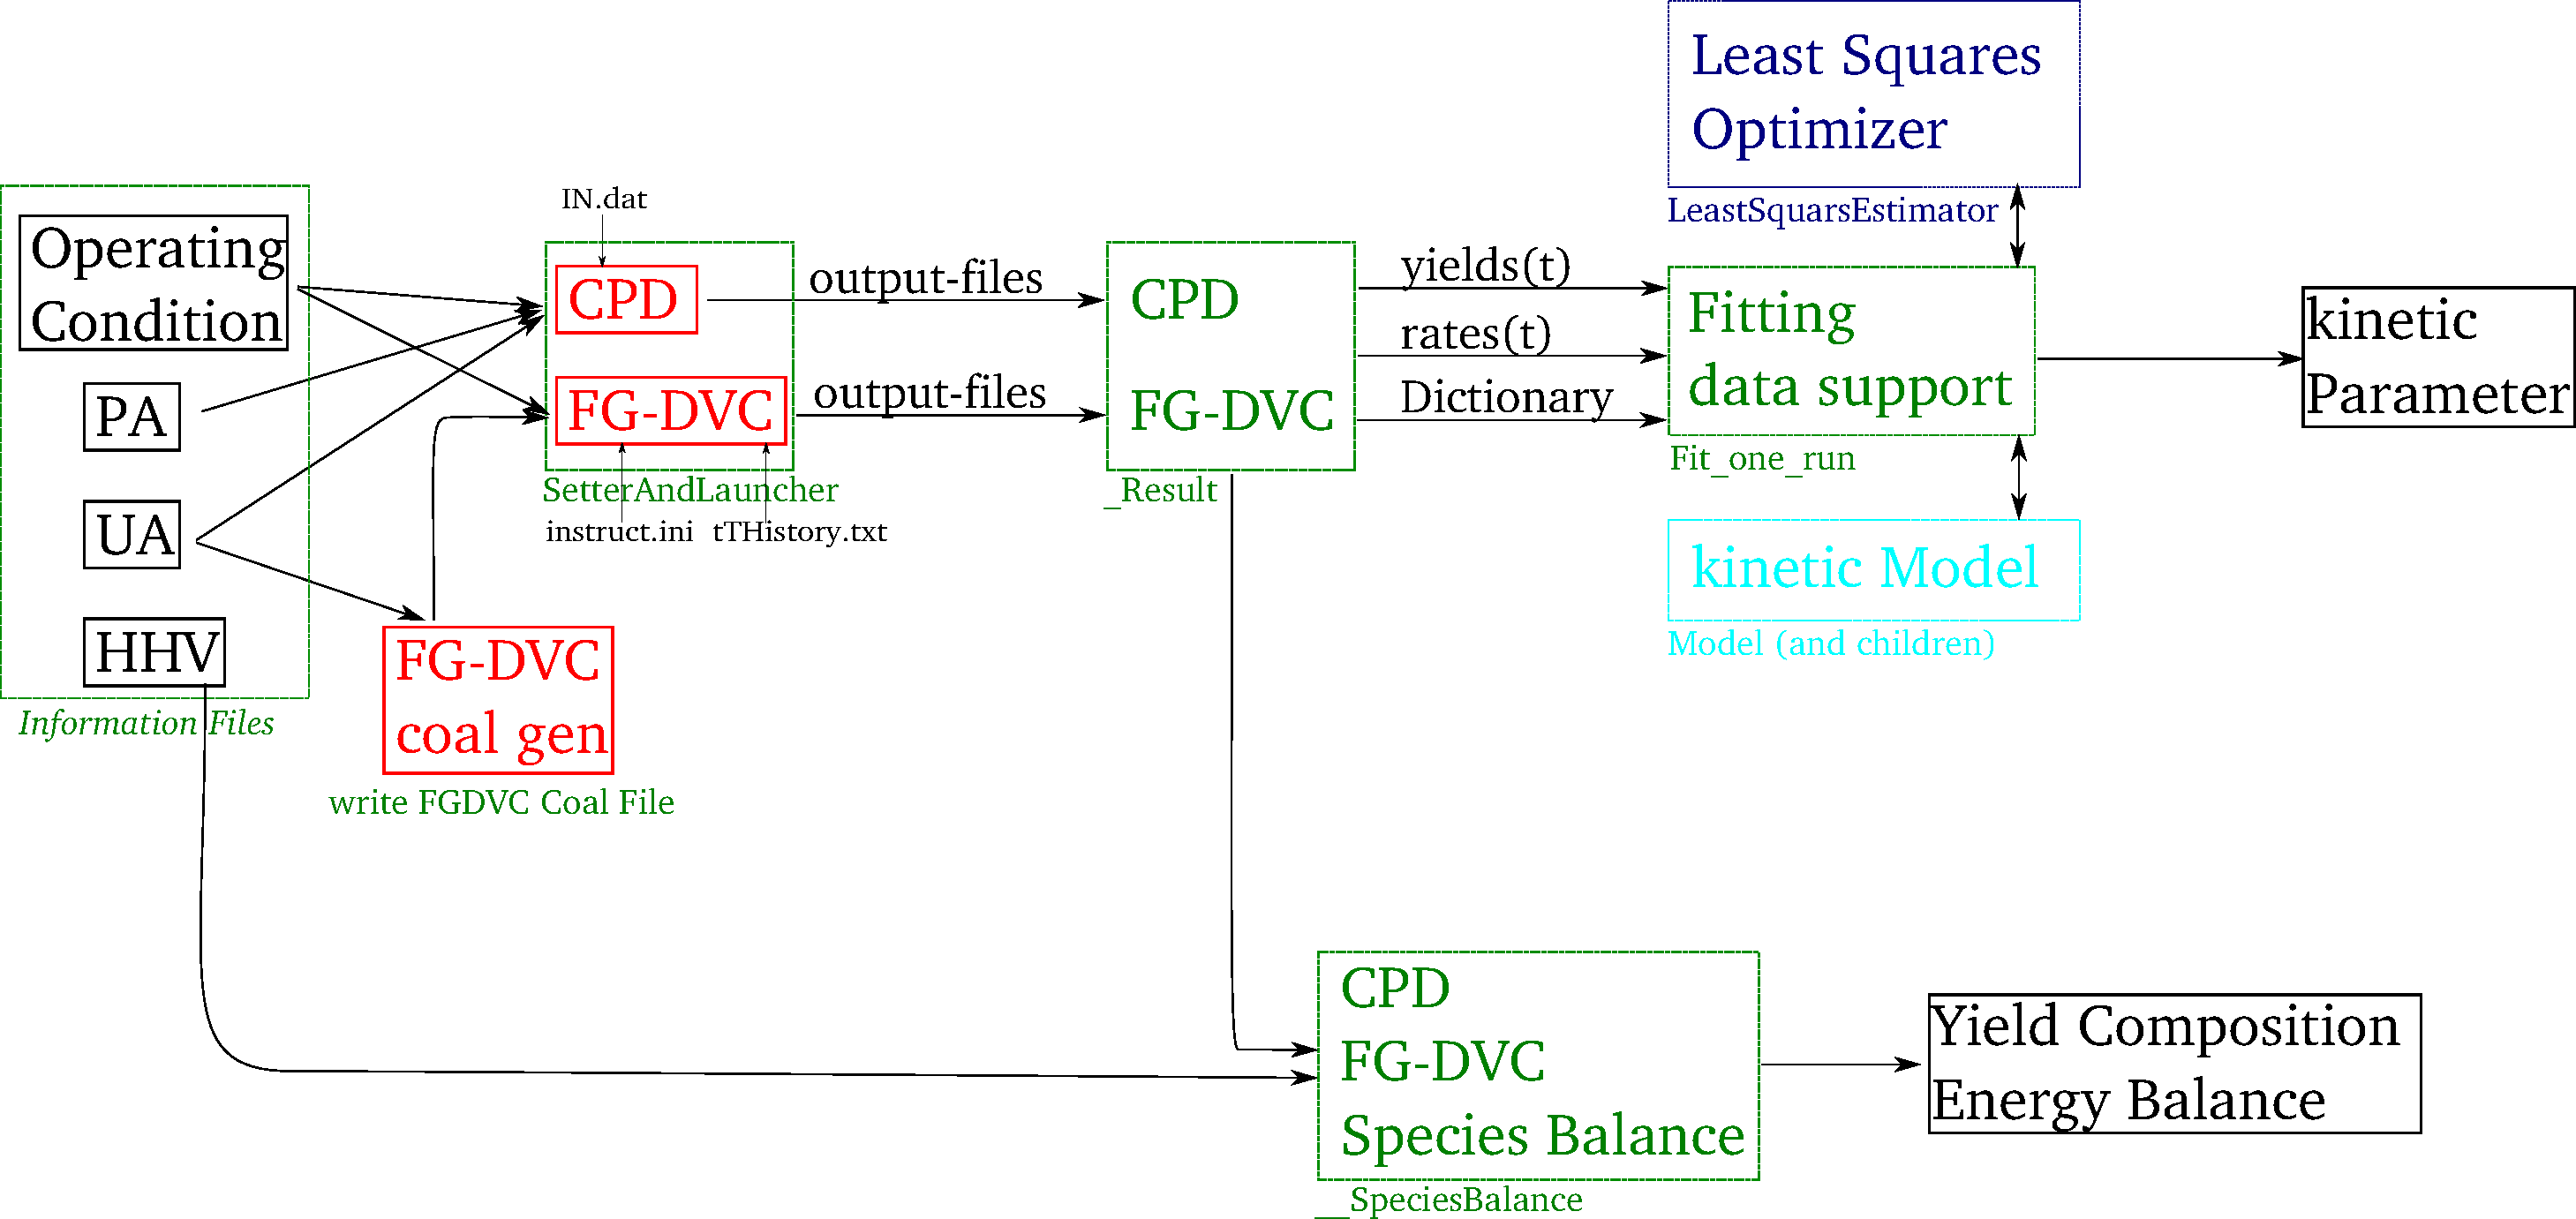
\includegraphics[width=22cm,angle=90]{Figures/Programstructure}
\caption{Overview of the program. The Optimization procedure is shown detailed in figure~\ref{F_OptimizationProc}.}
\label{F_Structure}
\end{figure}

\begin{figure}
\centering%\capstart
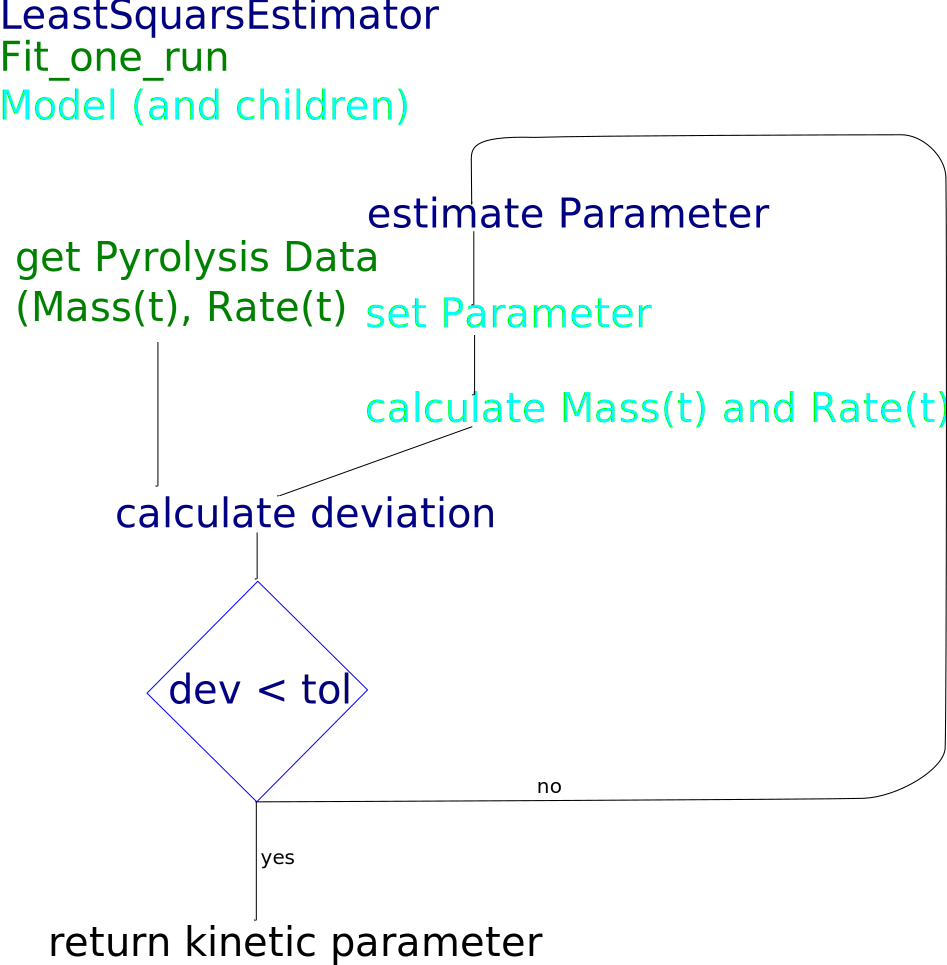
\includegraphics[height=9cm,angle=0]{Figures/FittingProcedure}
\caption{The optimization structure. The three classes \textit{LeastSquarsEstimator}, \textit{Fit\_one\_run} and \textit{Model} are marked with different colors like in Figure~\ref{F_Structure}. The Deviation is calculated with equation~\ref{E_LS}.}
\label{F_OptimizationProc}
\end{figure}

In figure~\ref{F_Structure} the external programs are colored in red, the PKP classes are in green, marked below with the class name or the relevant file name. Inputted, transfered or outputted data is in black.\\
So as first the specific user information about the operating conditions and the coal properties are imported using the reading classes contained in \emph{Information Files.py}.\\
Parts of this information are further used to write the input file for the \FGDVC coal generator\footnote{If chosen this way by the user. Otherwise also a selected \FGDVC library coal can directly be used to run \texttt{FG-DVC}. Then this step is not done.}, which is launched afterwards to generate the \FGDVC coal input files.\\

Afterwards the pyrolysis programs are launched automatically by PKP. The file \emph{IN.dat} is an input file for \CPD telling how the output files should be named. So the content in \emph{IN.dat} shouldn't be changed. The central input file for \FGDVC is the \emph{instruct.ini} which contains all information about the location of the coal file, the operating conditions and the numerical parameters. This file was generated by PKP before launching. The second input file for \FGDVC contains the temperature history. This file (named \emph{tTHistory.txt}, located in the \FGDVC main directory) was also written by PKP before each run.\\
The output files of the pyrolysis programs are read by their specific \emph{*\_Result} classes (e.g. \emph{CPD\_Result}). These classes save the information from the output files, contain a dictionary with the information which column contains which species and physical variable. The  \emph{*\_Result} classes also process the specific information (e.g. the modifications described in chapter~\ref{SS_Generate_Results}, or the transformation from ms into s in the \CPD output). Converting this pyrolysis program specific output shape into a general one has two main advantages. As this 'standard shaped' information are passed to the following fitting data class \emph{Fit\_one\_run}, is the fitting procedure working for the output of all pyrolysis programs the same way. The second advantage is, that for a modified output of a new version of a pyrolysis program just a new \emph{*\_Result} class needs to be added, modified for the new output shape.
Using the dictionaries has the advantage that the code is better readable, more robust against modifications and more general purpose. So in the program the yield of tar can be requested with \emph{self.Yield('Tar')} instead of using any number. A species must not have the same index in the output of the \emph{*\_Result} classes, which might also not work as the pyrolysis programs have different number of species in the yields (\FGDVC has 15 species in the yields, \CPD eight).\\

The fitting procedure is carried out using three classes: a Least Squares Estimator, a kinetic model and a class for the pyrolysis program results, see figure~\ref{F_Structure} and the more detailed figure~\ref{F_OptimizationProc}. Depending on the selected kinetic model and its parameter to fit one of the children classes (e.g. constant Rate, of the parent class model) is selected. As the initial guess of the parameter\footnote{defined in the code} is in the physical realistic range, this problem can be fitted with a gradient based optimizer. The optimizer class calculates the deviation, equation~\ref{E_LS} using the data from the \emph{Fit\_one\_run} class\footnote{which provides the pyrolysis program results} and the calculated yields of the model applying the current kinetic parameter.
The deviation allows the optimizer a new estimation of the parameter. This estimated parameter are passed to the kinetic model class, which sets these parameter for a further use of calculating the mass over time. This loop is repeated until the deviation is lower than the setted tolerance.\\

The species and energy balance is carried out with specific classes for \FGDVC and \texttt{CPD}. As these are straight forward analytical calculations, chapters~\ref{SSS_ConsEqCPD}~and~\ref{SSS_ConsEqFGDVC}, these classes just needs to be initialized with the right input parameter to output afterwards the results applying their private methods, see the \emph{PKP Code Documentation}.

\newpage
\bibliographystyle{plain}%plain, abbrv, alpha
\bibliography{bibo}
\end{document}
